\documentclass[11pt,a4paper,oneside]{memoir}

\chapterstyle{section}
\copypagestyle{centerruled}{ruled}
\makeevenfoot{centerruled}{}{\thepage}{}
\makeoddfoot{centerruled}{}{\thepage}{}

\usepackage{graphicx}
\usepackage{geometry}
\usepackage{hyperref}
\usepackage[table]{xcolor}
\usepackage[backend=biber,style=numeric,maxnames=4]{biblatex}
\usepackage{tabularx}
\usepackage{acro}
\usepackage{amsmath}

\newcolumntype{L}{>{\raggedright\arraybackslash}X}
\newcolumntype{C}{>{\centering\arraybackslash}X}
\def\tabularxcolumn#1{m{#1}}

\addbibresource{bibliography.bib}

\hypersetup{
	colorlinks=true,
	linkcolor=black,
	urlcolor=blue,
	citecolor=black,
}

\graphicspath{{figures/}}

\setsecnumdepth{subsection}

\setcounter{tocdepth}{2}

\acsetup{make-links,list/display=all}

\DeclareAcronym{sw}{
	short=SW,
	long=Software,
}

\DeclareAcronym{hw}{
	short=HW,
	long=Hardware,
}

\DeclareAcronym{fsm}{
	short=FSM,
	long=Finite-State Machine,
}

\DeclareAcronym{hdl}{
	short=HDL,
	long=\acl{hw} Description Language,
}

\DeclareAcronym{rtl}{
	short=RTL,
	long=Register-Transfer Level
}

\DeclareAcronym{hls}{
	short=HLS,
	long=High-Level Synthesis,
}

\DeclareAcronym{fpga}{
	short=FPGA,
	long=Field-Programmable Gate Array,
}

\DeclareAcronym{fifo}{
	short=FIFO,
	long=First-In First-Out,
}

\DeclareAcronym{lru}{
	short=LRU,
	long=Least Recently Used,
}

\DeclareAcronym{ram}{
	short=RAM,
	long=Random Access Memory,
	long-plural-form=Random Access Memories,
}

\DeclareAcronym{dram}{
	short=DRAM,
	long=Dynamic RAM,
}

\DeclareAcronym{bram}{
	short=BRAM,
	long=Block RAM,
}

\DeclareAcronym{axi}{
	short=AXI,
	long=Advanced eXtensible Interface,
}

\DeclareAcronym{raw}{
	short=RAW,
	long=Read After Write,
}

\DeclareAcronym{ii}{
	short=II,
	long=Initiation Interval,
}

\DeclareAcronym{l1}{
	short=L1,
	long=Level 1,
}

\DeclareAcronym{l2}{
	short=L2,
	long=Level 2,
}

\DeclareAcronym{api}{
	short=API,
	long=Application Programming Interface,
}

\DeclareAcronym{ipc}{
	short=IPC,
	long=Inter-Process Communication,
}

\DeclareAcronym{lsb}{
	short=LSB,
	long=Least Significant Bit,
}

\DeclareAcronym{msb}{
	short=MSB,
	long=Most Significant Bit,
}

\renewcommand*{\maketitle}%
{
	\newgeometry{left=2cm,right=2cm,top=3cm,bottom=3.5cm}

	\begin{center}
		\begingroup
		{\Huge\textbf{POLITECNICO DI TORINO}}\\[\baselineskip]
		\rule{\textwidth}{2pt}\par
		\vspace*{1em}
		{\LARGE\textbf{Master's Degree in Computer Engineering}}\\[\baselineskip]
		\vspace*{1em}
		{\Large\textbf{Master's Degree Thesis}}\\
		\vspace*{2cm}
		{\huge\textbf{Acceleration by Separate-Process Cache for
		Memory-Intensive Algorithms on \acs{fpga} via \acl{hls}}}\\
		\vspace*{1cm}
		
\includegraphics[width=.3\textwidth]{figures/polito-logo}
	\end{center}
	\vfill
	\begin{minipage}{0.4\textwidth}
		\begin{flushleft}
			{\Large
				\textbf{Supervisor}\\
				Prof.\ Luciano Lavagno
			}
		\end{flushleft}
	\end{minipage}
	\begin{minipage}{0.4\textwidth}
		\begin{flushright} 
			{\Large
				\textbf{Candidate}\\
				Giovanni Brignone\\
				ID: 274148
			}
		\end{flushright}
	\end{minipage}  
	\vspace*{2cm}
	\begin{center}
		{\Large\textbf{Academic year 2020-2021}}
	\end{center}
	\endgroup

	\restoregeometry 
}

\begin{document}
\pagestyle{empty}
\maketitle

\clearpage
\pagestyle{plain}

\frontmatter
\chapter*{Abstract}
The end of the Moore's Law validity is making the performance advance of
\acl{sw} run on general purpose processors more challenging than ever.
Since current technology cannot scale anymore it is necessary to approach the
problem from a different point of view: application-specific \acl{hw} can
provide higher performance and lower power consumption, while requiring higher
design efforts and higher deployment costs.

The problem of the high design efforts can be mitigated by the \acf{hls}, since
it helps improve designer productivity thanks to convenient \acl{sw}-like
tools.

The problem of high deployment costs can be tackled with \acp{fpga}, which allow
implementing special-purpose \acl{hw} modules on general-purpose underlying
physical architectures.

\bigskip
One of the open issues of \ac{hls} is the memory bandwidth bottleneck which
limits performance, especially critical in case of memory-bound algorithms.

\acp{fpga} memory system is composed of three main kinds of resources: registers,
\acp{bram} and external \acp{dram}.
Current \ac{hls} tools allow to exploit this memory hierarchy manually, in a
scratchpad-like fashion: the objective of this thesis work is to automate the
memory management by providing an easily integrable and fully customizable cache
system for \ac{hls}.

\bigskip
The proposed implementation has been developed using Vitis\texttrademark HLS
tool by Xilinx Inc..

The first development phase produced a single-port cache module, in the form of
a C++ class configurable through templates in terms of number of sets, ways,
words per line and replacement policy.
The cache lines have been mapped to \acp{bram}.
To obtain the desired performance, an unconventional (for \ac{hls}) multiprocess
architecture has been developed: the cache module is a separate process with
respect to the algorithm using it: the algorithm logic sends a memory access
request to the cache and reads its response, communicating through \acsp{fifo}.

\bigskip
In the second development phase, the focus was put on performance optimization,
in two dimensions: increasing the memory hierarchy depth by introducing a
\ac{l1} cache and increasing parallelism by enabling multiple ports.

The \ac{l1} cache is composed of cache logic inlined in the user algorithm: this
solution allows to cut the costs of \acp{fifo} communications. To keep \ac{l1}
cache simple it has been implemented with a write-through write policy,
therefore it provides advantages for read accesses only. It is configurable in
the number of lines and each line contains the same number of words of the
associated \ac{l2} cache.

The multi-port solution provides a single \ac{l2} cache accessible from multiple
\acp{fifo} ports, each of which can be associated with a dedicated \ac{l1}
cache.
It is possible to specify the number of ports through a template parameter and
it typically corresponds to the unrolling factor of the loop in which the cache
is accessed.

\bigskip
In order to evaluate performance and resource usage impact of the developed
cache module, multiple algorithms with different memory access patterns have
been synthesized and simulated, with all data accessed to \ac{dram} (performance
lower bound), to \ac{bram} (performance higher bound) and to cache (with
multiple configurations).

\vfill
\pagebreak

\tableofcontents*
\vfill
\pagebreak

\listoffigures
\vfill
\pagebreak

\listoftables
\vfill
\pagebreak

\printacronyms[heading=chapter,name={List of Acronyms}]
\vfill
\pagebreak

\clearpage
\pagestyle{centerruled}

\mainmatter
\chapter{Background}
The literature about cache systems, the \acl{hls} state of the art and an
analysis of the resources available on board modern \acp{fpga} are the
fundamental background for this thesis work.

\section{Cache}
Memory devices are crucial components of computing systems as they can pose an
higher bound in terms of performance, especially when executing memory-intensive
algorithms.
The ideal memory should be fast, large and cheap, but current technology forces
the designer to choose a trade-off between the metrics.

A common solution to this problem is to set up a memory hierarchy in
which fast but small memories are paired with large but slow memories, which
allows getting good performance on average while containing costs.

This hierarchy can be managed by two main approaches:
\begin{itemize}
	\item \emph{Scratchpad}: different memories belongs to different
		addressing spaces: the user is in charge of manually choosing
		what memory to access: this approach allows to optimally
		exploit the hierarchy at the cost of high design effort.
	\item \emph{Cache}: different memories belongs to the same addressing
		space: the system automatically uses the whole hierarchy,
		exploiting spatial locality (accessed data is likely physically
		close to previously accessed data) and temporal locality
		(accessed data has likely recently been accessed), which are
		typical of many algorithms.
\end{itemize}

\subsection{Structure}
A cache memory is logically split into \emph{sets} containing \emph{lines} (or
\emph{ways}) which are in turn made up of \emph{words}, as shown in
Figure~\ref{fig:cache_logic_structure}.

\begin{figure}[!htb]
	\centering
	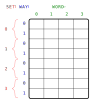
\includegraphics[width=.5\textwidth]{cache_logic_structure}
	\caption{Cache logic structure.}
	\label{fig:cache_logic_structure}
\end{figure}

Whenever a word $w$ is requested, there are two possibilities:
\begin{itemize}
	\item \emph{Hit}: $w$ is present in the cache: the request can be
		immediately fulfilled.
	\item \emph{Miss}: $w$ is not present in the cache: it is necessary to
		retrieve it from lower level memory before fulfilling the
		request.
\end{itemize}
During the data retrieving, a cache line is filled with a block of contiguous
words loaded from the lower level memory, trying to exploit spatial locality of
future accesses, while mapping policies and replacement policies determine which
cache line to overwrite, trying to exploit temporal locality.

If the cache memory is writable, data consistency is ensured by a consistency
policy.
\subsection{Policies}
\subsubsection{Mapping policy}
The mapping policy is in charge of statically associating a lower level memory
line to a cache set.

The \emph{set associative} policy is the most common mapping policy: given a
cache memory with $s$ sets of $w$ words, the word address (referred to the lower
level memory) bits are split into three parts (as shown in
Figure~\ref{fig:address_partitioning}):
\begin{enumerate}
	\item $\log_2(w)$: offset of the word in the line.
	\item $\log_2(s)$: set.
	\item Remaining \acsp{msb}: tag identifying the specific line.
\end{enumerate}

\begin{figure}[!htb]
	\centering
	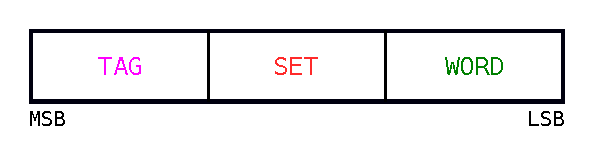
\includegraphics[width=.5\textwidth]{address_partitioning}
	\caption{Set associative policy address bits meaning.}
	\label{fig:address_partitioning}
\end{figure}

Special cases of this policy are:
\begin{itemize}
	\item \emph{Direct mapped} policy: each set is composed of a single
		line: the set bits identify a specific cache line, therefore
		there is no need for a replacement policy.
	\item \emph{Fully associative} policy: there is only a single set,
		therefore the line is fully determined by the replacement
		policy.
\end{itemize}

\subsubsection{Replacement policy}
The replacement policy is in charge of dynamically associating a lower level
memory line to a cache line of a set.

Multiple solutions of this problem have been developed, trying to maximize
the temporal locality exploitation.
Among the most commonly used solutions there are:
\begin{itemize}
	\item \emph{\acl{fifo}}: the line to be replaced is the first
		one that has been inserted to the cache.
	\item \emph{\acl{lru}}: the line to be replaced is the one
		that has least recently been accessed.
\end{itemize}

\subsubsection{Consistency policy}
The consistency policy is in charge of ensuring data consistency between
memories belonging to different hierarchy levels.

The most common solutions to this problem are:
\begin{itemize}
	\item \emph{Write-back}: write accesses are performed to the highest
		level memory and lower level memories are updated when the cache
		line is replaced only.
	\item \emph{Write-through}: each write access is propagated along the
		whole hierarchy.
\end{itemize}

\subsection{Benefits}
A two-level memory hierarchy is composed of a \ac{l1} cache memory (access time:
$t_{L1}$; access energy: $E_{L1}$) and a \ac{l2} memory (access time: $t_{L2}$;
access energy: $E_{L2}$), with $t_{L1} << t_{L2}$ and $E_{L1} << E_{L2}$.

This memory hierarchy is accessed $n_{\text{tot}}$ times and $n_{\text{hit}}$
of these accesses are cache hits.

\bigskip
The \emph{hit ratio} is defined as: 
\begin{equation}
	H := \frac{n_\text{hit}}{n_{\text{tot}}}
\end{equation}

The \emph{average access time} and \emph{energy} are defined as:
\begin{equation}\label{eq:avg_acc}
	\begin{cases}
	\overline{t}(H) := H t_{\text{L1}} + (1 - H) t_{\text{L2}} \\
	\overline{E}(H) := H E_{\text{L1}} + (1 - H) E_{\text{L2}} \\
	\end{cases}
\end{equation}

Equation~\ref{eq:avg_acc} shows the criticality of the \emph{hit ratio}: the
performance and power consumption advantages provided by the cache are
significant if and only if $H$ is sufficiently near to 1.

\section{\acl{fpga}}
\aclp{fpga} are integrated circuits able to implement special purpose circuits
described in \ac{hdl}, thanks to their programmable logic blocks and
interconnections.
\subsection{Memory system}
A \ac{fpga} memory system is typically made up of:
\begin{itemize}
	\item Registers: the fastest but most expensive memories, therefore
		they are only a few.
	\item \acp{bram}: on chip \acp{ram} accessible through simple and fast
		interface.
	\item External \acp{dram}: off chip \acp{dram} accessible through
		complex and slow interface (e.g.\ \acs{axi}).
\end{itemize}

\section{\acl{hls}}
\acf{hls} is an Electronic Design Automation technique aimed at translating an
algorithm description in a high-level \acl{sw} programming language (such as C
and C++) into a \ac{hdl} description.

\ac{hls} allows designing more complex systems in less time, compared to
\ac{hdl} design, moreover makes the \acl{hw} and \acl{sw} co-design easier, at
the cost of limited low-level control.

This Section is mainly referred to
\emph{Vitis\texttrademark~HLS}~\cite{vitisug}, but most currently available
\ac{hls} commercial tools provide equivalent features.

\subsection{Workflow}
The typical \ac{hls} workflow consists of:
\begin{enumerate}
	\item \emph{\ac{sw} implementation}: the top-level entity is a C
		function: the function arguments are the entity ports and the
		functionality is implemented in \ac{sw}; in order to guarantee
		synthesizability some constraints should be respected (e.g.\ no
		dynamic memory allocation).
	\item \emph{\ac{sw} verification}: the testbench can be developed as a
		simple main function which calls the top-level entity function,
		therefore the functionality is verified like any \ac{sw}: it is
		possible to exploit traditional tools (e.g.\ debuggers, print
		statements\ldots).
	\item \emph{\ac{hw} synthesis}: the synthesizer generates a \ac{rtl}
		description of the top-level entity. It is possible to generate
		different architectures by setting up some parameters through
		dedicated directives.
	\item \emph{\ac{hw} verification}: the \ac{rtl} description is
		simulated, to make sure that \ac{sw} and \ac{hw} outputs match.
\end{enumerate}

\subsection{Optimization techniques}
\ac{hls} tools provide different optimization techniques which can be set up by
means of compiler directives.
\subsubsection{Pipelining}
Given a set of sequential stages (e.g.\ A, B and C of Figure~\ref{fig:pipeline})
which compose an operation (e.g.\ A + B + C of Figure~\ref{fig:pipeline}) which
has to be executed multiple times, the pipelining technique inserts pipeline
registers at the output of each stage, so that each stage can run in parallel
on different input data (e.g.\ at the third clock cycle, while C is processing
first input, B is processing second input and A is processing third input).
The introduced parallelism allows to increase the throughput at a limited
additional area cost (only pipeline registers and a \acs{fsm} are required).

The throughput is determined by the interval (expressed in number of clock
cycles) between the beginning of two consecutive executions of the operation,
which is called \ac{ii}.
The optimal pipeline has an \ac{ii} equal to one: at the steady state, one output
per clock cycle is produced.

\bigskip
The pipelining can be performed at instruction level, within a loop or a
function, or at function level (in \ac{hls} terminology this particular kind of
pipelining is called \emph{Dataflow}).

\begin{figure}[!htb]
	\centering
	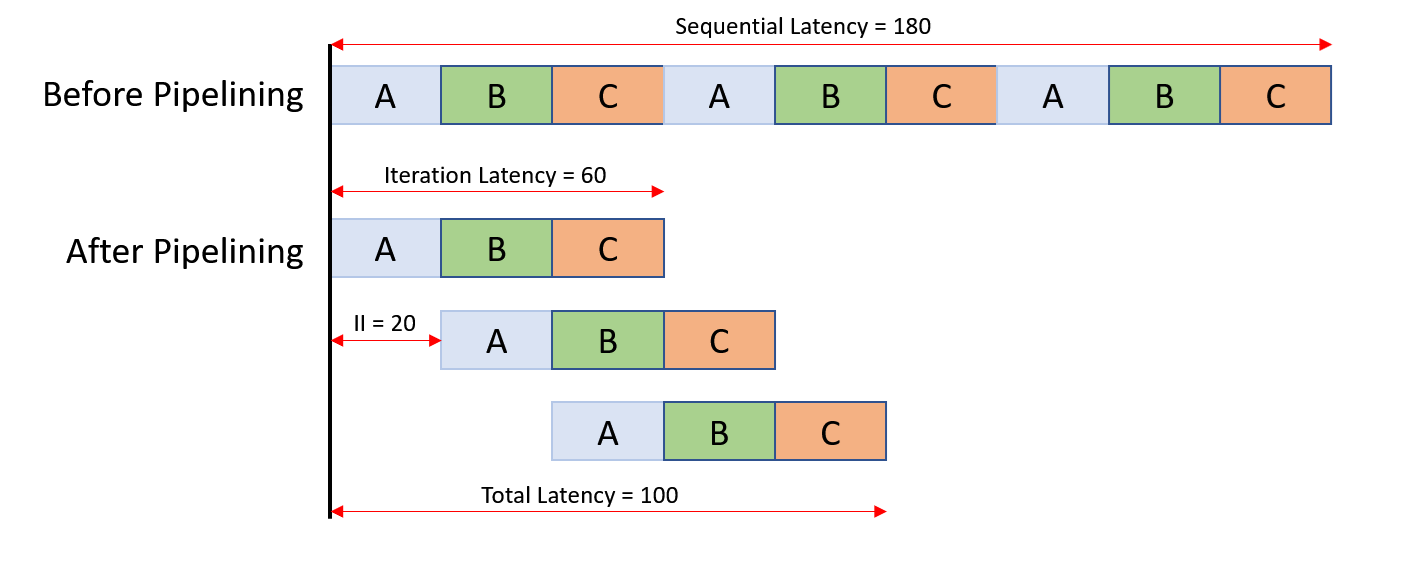
\includegraphics[width=.8\textwidth]{pipelining}
	\caption{Pipelining example.}
	\label{fig:pipeline}
\end{figure}

\subsubsection{Loop unrolling}
The logic of a rolled loop allows the execution of one iteration at a time: if
the loop iterates $N$ times and each iteration has a latency $L_{it}$, the
total loop latency is equal to ${L_{loop, rolled} := N \cdot L_{it}}$.

The loop unrolling technique instantiates the logic for executing $f$ iterations
at a time (where $f$ is the unrolling factor).
If there are no dependencies between different iterations, the latency of the
unrolled loop is: ${L_{loop, unrolled}(f) := \frac{N}{f} \cdot L_{it}}$.

\bigskip
Loop unrolling can improve both latency and throughput, but it is expensive in
terms of resource usage, since they are multiplied by $f$.

\begin{figure}[!htb]
	\centering
	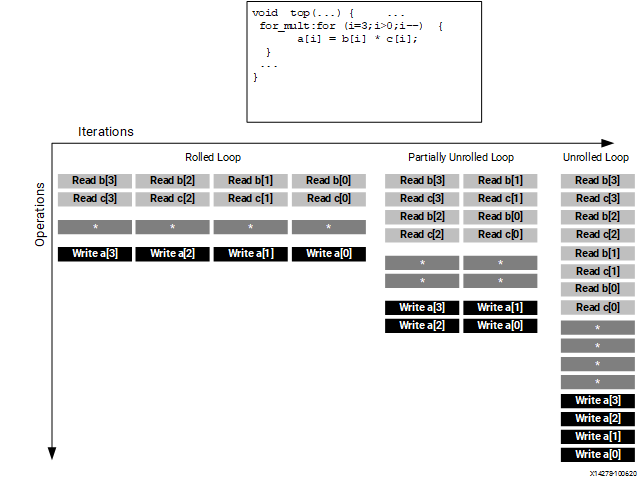
\includegraphics[width=.8\textwidth]{unroll}
	\caption{Loop unrolling example.}
\end{figure}

\subsubsection{Memory optimizations}
\begin{itemize}
	\item \underline{On-chip memory:}
		\begin{itemize}
			\item \textbf{Array partitioning}: given a partitioning
				factor $f$, an array is split into $f$
				portions, each one mapped to a dedicated memory
				element.

				This allows multiple concurrent accesses to the
				same array, at the cost of higher memory
				elements usage.

				Figure~\ref{fig:array_partitioning} shows
				different partitioning modes.
				\begin{figure}[!htb]
					\centering
					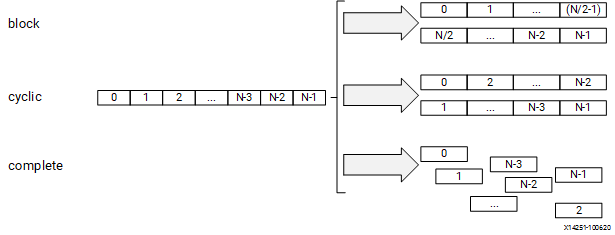
\includegraphics[width=.8\textwidth]{
						array_partitioning}
					\caption{Array partitioning examples.}
					\label{fig:array_partitioning}
				\end{figure}
		\end{itemize}
	\item \underline{Off-chip memory}:
		\begin{itemize}
			\item \textbf{Interface widening}: multiple data
				elements are packed into a single bigger word,
				to perform multiple accesses at the same time.
			\item \textbf{Burst accesses}: multiple memory accesses
				are aggregated into \ac{axi} bursts to reduce
				overall latency and improving throughput.
				\begin{figure}[!htb]
					\centering
					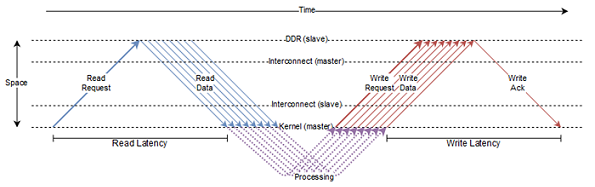
\includegraphics[width=.9\textwidth]{
						burst}
					\caption{Burst read and write example.}
				\end{figure}
		\end{itemize}
\end{itemize}

\chapter{Development}
\ac{hls} tools are currently unable to automatically exploit the memory
hierarchy present on \acp{fpga}: the only way to take advantage of
them is the manual management in a \emph{scratchpad}-like manner, which
requires additional design and verification efforts.

The proposed solution \textbf{automates the low-level memory management}
through a cache module for \ac{hls}, which works as an interface with the
off-chip \ac{dram} (accessible through an \ac{axi} bus) and stores its data to
on-chip \acp{bram} and registers.

\section{Overview}
The proposed cache module has the \textbf{dual purpose} of:
\begin{itemize}
	\item \emph{Reducing the number of \ac{dram} accesses}: misses only
		needs to access \ac{dram}.
	\item \emph{Optimizing \ac{dram} accesses}: lines are accessed in
		bursts through a widened memory interface.
\end{itemize}

\acp{fpga} provide multiple \ac{dram} ports and \ac{hls} can assign each array
to a different port: this allows implementing \textbf{array-specific} caches,
which in general can be easily tuned to reach high hit ratios, since access
patterns to a single array are usually regular and there is no interference
between accesses to different arrays.

\bigskip
A special attention has been put on \textbf{user-friendliness}:
\begin{itemize}
	\item \emph{Configurability}: cache characteristics can be set through
		parameters.
	\item \emph{Integrability}: cache can be inserted into existing designs
		without requiring many changes.
	\item \emph{Observability}: critical cache data (e.g.\ hit ratio) can
		be profiled during \ac{sw} simulation for easing the cache
		parameters tuning.
\end{itemize}

\subsection{Ma's cache}
Liang Ma et al.\ proposed a \texttt{C++} cache implementation~\cite{liang}
compatible with the \emph{SDAccel\texttrademark} \ac{hls} tool.

It is an array-specific cache module in the form of different \texttt{C++}
classes: each of them implements an access type (read only/write only and read
write) and a mapping policy (direct mapped and set associative).

To improve the \emph{integrability} the \texttt{operator[]} has been overloaded
so that the cache object can be accessed in the same way as array variables,
minimizing the required changes to the code which integrates the cache.

\bigskip
This architecture is \textbf{inlined}: the cache logic is directly inserted in
the user algorithm logic.
This is the major limitation of this solution, since the additional logic
inserted in the algorithm may make it too complex and worsen the generated
circuit performance.

\subsection{Proposed solution}
The primary goal is to develop the \emph{Basic cache}, a cache architecture
which runs in a separate process with respect to the application using it,
trying to solve the main limitation of \emph{Ma's cache}: the application logic
cluttering due to the inlining.

This architecture has been then optimized in two dimensions:
\begin{itemize}
	\item \emph{Multi-levels cache}: a \ac{l1} cache are added to the cache
		hierarchy, with the objective of further reducing memory access
		latency.
	\item \emph{Multi-ports cache}: multiple cache access points are added
		to the cache, each one with a dedicated \ac{l1} cache, so that
		multiple requests can be served in parallel.
\end{itemize}

\clearpage

\section{Basic cache}
The \emph{Basic cache} is aimed at solving the main limitation of \emph{Ma's
cache}: application logic cluttering due to inlining.

\subsection{Architecture}
The fundamental idea behind the \emph{Basic cache} is that the cache logic is
inserted in a separate process with respect to the application logic accessing
it (Figure~\ref{fig:single_proc_basic_arch}): this isolation should make the
cache always perform in the same manner, while keeping the application logic as
clean as possible, since it would only have to write requests to cache and read
its responses, instead of integrating its whole logic.

\begin{figure}[!htb]
	\centering
	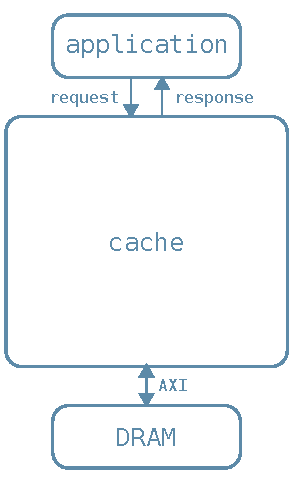
\includegraphics[width=.3\textwidth]{single_proc_basic_arch}
	\caption{\emph{Single-process Basic cache} architecture.}
	\label{fig:single_proc_basic_arch}
\end{figure}

\subsubsection{Functionality}
If application $A$ needs to access the array associated with the cache $C$:
\begin{enumerate}
	\item $A$ sends the access request to $C$: operation (i.e.\ read or
		write), address and (in case of write access) data.
	\item $C$ receives the request and checks if the requested address
		causes a miss.
	\item (in case of miss) $C$ prepares its \ac{bram} memory for fulfilling
		the requested access:
		\begin{itemize}
			\item (if needed) writes back to \ac{dram} the \ac{bram}
				line to be replaced.
			\item reads from \ac{dram} the requested line and store
				it to \ac{bram}.
		\end{itemize}
	\item $C$ performs the requested access to \ac{bram} and (in case of
		read request) sends requested data to $A$.
\end{enumerate}

\subsubsection{Characteristics}
The \emph{Basic cache} is compliant with the set associative mapping policy and
the write-back consistency policy.
It is configurable in terms of:
\begin{itemize}
	\item Word type and number of words per line.
	\item Number of sets and ways (therefore, it is possible to obtain a
		fully associative policy by setting the number of sets to 1 or
		a direct mapped policy by setting the number of ways to 1).
	\item Replacement policy (\acl{lru} or \acl{fifo}).
\end{itemize}

\subsubsection{Single-process Basic cache}
The \emph{Single-process Basic cache} is composed of a single pipelined process
which performs all the cache functionalities.

This process can be pipelined with an \ac{ii} equal to 1 when memory accesses
are Read-Only and a cache line can fit a single \ac{axi} transaction (i.e.\
line is not bigger than the maximum \ac{axi} interface width: 512 or 1024 bits
typically, depending on the specific device).

Write accesses generate some dependencies on the \ac{axi} interface, while large
cache lines require multiple \ac{axi} transactions: both of them cause an
increase of the process \ac{ii}, ruining cache performance.

\subsubsection{Multi-processes Basic cache}
The \emph{Multi-processes Basic cache} splits cache into two processes
(Figure~\ref{fig:multi_proc_basic_arch}):
\begin{itemize}
	\item \emph{Core} process: manages communication with application and
		keeps cache data structures up to date.
	\item \emph{Memory interface} process: deals with the \ac{axi}
		interface.
\end{itemize}

This architecture is aimed at solving the performance limitations of the
\emph{Single-process Basic cache}: it manages to pipeline the \emph{core}
process with an \ac{ii} equal to 1, even in case of write accesses or long
lines, since the \ac{axi} interfacing resides in the separate \emph{memory
interface} process.

The latency of the response to a hitting request depends on the \emph{core}
process only, therefore with this solution the best performance is achieved in case
of writable caches too.

\begin{figure}[!htb]
	\centering
	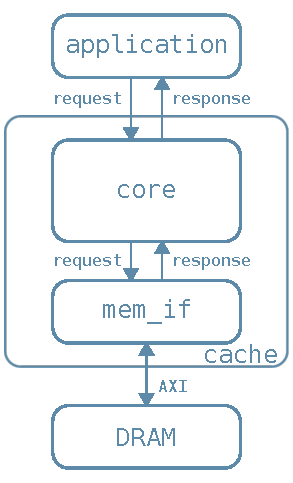
\includegraphics[width=.3\textwidth]{multi_proc_basic_arch}
	\caption{\emph{Multi-processes Basic cache} architecture.}
	\label{fig:multi_proc_basic_arch}
\end{figure}

\subsection{Implementation}
The \emph{Basic cache} is implemented in the form of a
\texttt{C++14}~\cite{cpp14} class, compatible with
\emph{Vitis\texttrademark~HLS~2021.1}.
All the configurable parameters are set through class template arguments.

The cache class is logically split into two parts:
\begin{itemize}
	\item \emph{Internals}: cache functionalities.
	\item \emph{Interface}: \acsp{api} for managing requests and responses
		from application side.
\end{itemize}

\subsubsection{Internals}
The \emph{Internals} implementation differs between the \emph{Single-process}
and the \emph{Multi-processes} implementations:
\begin{itemize}
	\item \emph{Single-process Basic cache}: single process which
		implements all the cache functionalities.
	\item \emph{Multi-processes Basic cache}:
		\begin{itemize}
			\item \emph{Core} process: same as \emph{Single-process
				Basic cache} process, but it does not
				directly access the \ac{axi} bus: it issues
				requests to the \emph{memory interface} process
				through \acp{fifo}.
			\item \emph{Memory interface} process: it accesses the
				\ac{axi} bus as requested by the \emph{core}
				process.
		\end{itemize}
\end{itemize}

\emph{Single-process Basic cache}, with respect to the \emph{Multi-processes}
one, requires lower resource usage and better performance, when it is possible
to schedule its process with an \ac{ii} equal to 1 (read-only accesses with
line not larger than the maximum \ac{axi} interface bitwidth): therefore it is
automatically instantiated whenever it is convenient.

\paragraph{Process modeling}
\ac{hls} is intended for synthesizing sequential \acl{sw} code, therefore it has
been necessary to develop a novel technique for modeling multiprocess designs.

A process is modeled as an infinite loop and the parallelism between multiple
processes is modeled differently depending on the compilation target:
\begin{itemize}
	\item \emph{\ac{sw} simulation}: each process is mapped to a
		\texttt{std::thread}.
	\item \emph{\ac{hw} synthesis}: each process is a dataflow function, in
		a dataflow region with the \texttt{disable\_start\_propagation}
		option disabled (which allow each function to run in parallel,
		without waiting for the completion of previous ones).
\end{itemize}
The distinction between simulation and synthesis code can be performed through
the ``\texttt{\#ifdef \_\_SYNTHESIS\_\_}'' preprocessor directive.

Different processes can communicate by means of \acp{fifo} (\texttt{hls::stream}
provided by Vitis\texttrademark HLS), which allow unidirectional point-to-point
communication between two processes. It is possible to insert multiple
\acp{fifo} between each process, in both directions, therefore allowing to
set up duplex communication.

Since \texttt{hls::stream} provides blocking operations, these \acp{fifo} can
be also used for synchronization purposes.

\paragraph{Dataflow checking}
Alternatively executing the \emph{Multi-processes} or the \emph{Single-process}
code with traditional \texttt{if} statements would generate errors during the
synthesis, particularly in the \emph{Dataflow check} step (which checks if each
\texttt{hls::stream} has a single reader and a single writer): the compiler
builds both branches of the \texttt{if} statements, independently of the fact
that one of them is never executed.

\bigskip
The problem has been solved through a wrapper class, which conditionally
includes a \texttt{hls::stream} object, exploiting the template specialization
mechanism.

\paragraph{Arrays partitioning}
Cache memory (which stores the actual data) must be accessed one line per clock
cycle: it is mapped to a \ac{bram} array cyclically partitioned with a factor
equal to the number of lines.

Helper data (e.g.\ \texttt{tag}, \texttt{valid}, \texttt{dirty}\ldots) is stored
to completely partitioned arrays, mapped to registers, in order to avoid
dependencies as much as possible and get the best performance.

\paragraph{\acl{raw} dependencies}
The cache process \ac{ii} is limited by the \ac{raw} dependencies on the cache
lines, therefore the \emph{\ac{raw} cache} has been developed: it is a
single-line cache which provides the functions:
\begin{itemize}
	\item \texttt{get\_line}: in case of hit, read the \emph{\ac{raw}
		cache} line; in case of miss, read the cache line.
	\item \texttt{set\_line}: write both the \emph{\ac{raw} cache} line and
		the cache line.
\end{itemize}

Cache memory is always accessed through the \emph{\ac{raw} cache} and the
\texttt{set\_line} function is called once per iteration at most: if a cache
line has been written, it is impossible that it is read in the next iteration,
since the \ac{raw} cache would hit and return its line. This allows to falsify
the \ac{raw} dependency of distance of 1 on the cache memory, making it
possible to schedule the cache process with an \ac{ii} equal to 1.

\subsubsection{Interface}
\emph{Interface} provides \acsp{api} for managing requests and responses from
application to cache:
\begin{itemize}
	\item \texttt{get}: send a read request and read the response.
	\item \texttt{set}: send a write request.
\end{itemize}
To improve user-friendliness, similarly to \emph{Ma's cache}, the
\texttt{operator[]} has been overloaded so that a cache object can be used as a
traditional array (e.g.\ \texttt{val~=~cache[i]} calls
\texttt{val~=~cache.get(i)} and \texttt{cache[i]~=~val} calls
\texttt{cache.set(i,~val)}).

\iffalse
\begin{table}
	\begin{center}
		\begin{tabularx}{\textwidth}{LCC}
			\hline
			\rowcolor{gray!50}
			& \textbf{Single-process basic implementation} &
			\textbf{Ma's implementation} \\
			\hline
			\textbf{Integration with algorithm} & Separate process &
			Inlined \\
			\rowcolor{gray!25}
			\textbf{Underlying memory} & Single \ac{dram} array &
			Single \ac{dram} array \\
			\textbf{Configurability} & Template arguments &
			Template arguments and dedicated classes \\
			\rowcolor{gray!25}
			\textbf{\texttt{operator[]} overload} & Array-like &
			Array-like \\
			\hline
		\end{tabularx}
	\end{center}
	\caption{Comparison between basic single-process and Ma's
	implementations.}
	\label{tab:basic_vs_liang}
\end{table}
\fi
\clearpage

\section{Multi-levels cache}
The \emph{Multi-levels cache} purpose is to improve the memory hierarchy
performance by adding a faster \ac{l1} cache memory on top of it.

\subsection{Architecture}
The \ac{ipc} (i.e.\ \ac{fifo} accesses) introduces an overhead at each memory
access, therefore the \ac{l1} cache is inlined in the application logic
(Figure~\ref{fig:l1_arch}), so that there is no need of any \ac{ipc} mechanism.

In order not to fall into the same cluttering issues of \emph{Ma's cache}, the
\ac{l1} cache is kept as simple as possible:
\begin{itemize}
	\item Mapping policy: direct-mapped.
	\item Consistency policy: write-through.
\end{itemize}

The write-through consistency policy discards any advantage for write accesses,
but given that simplicity is a priority and read accesses are usually much more
frequent than write accesses, this has been considered the best trade-off.

\begin{figure}[!htb]
	\centering
	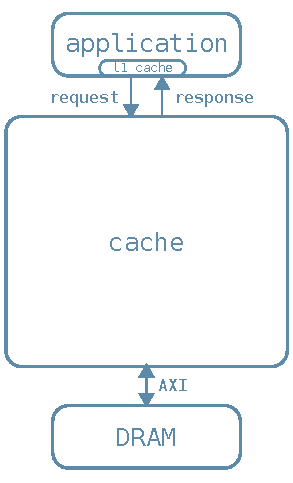
\includegraphics[width=.3\textwidth]{l1_arch}
	\caption{\emph{Multi-levels cache} architecture.}
	\label{fig:l1_arch}
\end{figure}

\subsection{Implementation}
The \emph{Multi-level cache} has been implemented adding the \ac{l1} cache to
the \emph{Basic cache}.
It is possible to configure the number of \ac{l1} cache lines through the
\texttt{L1\_CACHE\_LINES} template parameter, therefore by setting it to 0 the
resulting architecture is equivalent to the \emph{Basic cache}.

\subsubsection{Internals}
The only difference with respect to the \emph{Basic cache} implementation is
that the response to a read request does not send a single word, but a whole
cache line (therefore the data \ac{fifo} flowing from cache to application
has been widened accordingly).

\subsubsection{Interface}
The \ac{l1} cache is contained in the \emph{Interface}: the newly introduced
\texttt{get\_line} function receives an address $A$ in input and it returns the
line to which $A$ belongs.
In particular, it first checks if $A$ hits in the \ac{l1} cache: if so it reads
the data from the \ac{l1} cache, otherwise it issues the request to the \ac{l2}
cache.

\bigskip
It is still possible to use the same \emph{Basic cache} \acp{api}, which have
been updated to support the \ac{l1} cache:
\begin{itemize}
	\item \texttt{get}: it calls the \texttt{get\_line} function and then
		returns the requested word.
	\item \texttt{set}: it sets \ac{l1} cache line to dirty, if it hits, and
		it issues the request to the \ac{l2} cache.
\end{itemize}

\clearpage

\section{Multi-ports cache}
Most algorithms contain a loop which performs different operations, including
memory accesses.
\ac{hls} provides two main ways for optimizing loops: \emph{Pipelining} and
\emph{Unrolling}.

The \emph{Basic} and \emph{Multi-levels} caches complete one access per clock
cycle, at the steady state, in case of hit, therefore thery are suitable for
the use in pipelined loops, but not in unrolled loops, which require multiple
concurrent accesses.

The \emph{Multi-ports cache} is aimed at allowing multiple concurrent accesses
to better support loop unrolling.

\subsection{Architecture}
The \emph{Multi-ports cache} is characterized multiple access ports
(Figure~\ref{fig:multi_ports_arch}).

Each port has dedicated logic for accessing the \ac{l2} cache and an independent
\ac{l1} cache.
\ac{l1} caches comply with the write-through consistency policy, therefore to
guarantee coherency between the multiple caches it is enough to inform all the
\ac{l1} caches about write accesses, so that they invalidate their line in case
of hit.

\begin{figure}[!htb]
	\centering
	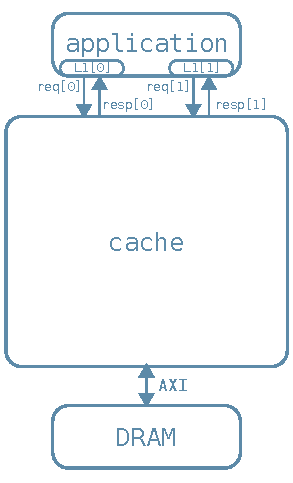
\includegraphics[width=.3\textwidth]{multi_ports_arch}
	\caption{\emph{Multi-ports cache} architecture.}
	\label{fig:multi_ports_arch}
\end{figure}

\subsection{Implementation}
\subsubsection{Internals}
\subsubsection{Interface}
\paragraph{Port binding}


\chapter{Results}
\section{Matrix multiplication}
\section{Bitonic sorting}
\section{Lucas-Kanade}

\chapter{Conclusion}

\backmatter

\printbibliography

\end{document}

